\documentclass[12pt]{report}

%\usepackage{titleps}
\usepackage{fancyhdr}
\usepackage{graphicx}
\usepackage[spanish]{babel}
\usepackage[utf8]{inputenc}
\usepackage{subfigure} 
\usepackage{todonotes}


\pagestyle{myheadings}
\pagestyle{fancy}
\fancyhf{}
\setlength{\headheight}{33pt}
\renewcommand{\headrulewidth}{2pt}
\renewcommand{\footrulewidth}{2pt}

\fancyhead[L]{
\includegraphics[width=1cm]{LogoUTN.png}}
\fancyhead[C]{}
\fancyhead[R]{Universidad Tecnológica Nacional - Facultad regional Córdoba}
\fancyfoot[R]{\thepage}



\begin{document}


\begin{titlepage}

    \begin{center}
    \vspace*{-1in}
    \begin{figure}[htb]
    \begin{center}
    
\includegraphics[width=8cm]{LogoUTN.png}
    \end{center}
    \end{figure}
    
    FACULTAD REGIONAL CÓRDOBA\\
    \vspace*{0.15in}
    DEPARTAMENTO DE INGENIERÍA ELECTRÓNICA \\
    \vspace*{0.6in}
    \begin{large}
    PROYECTO FINAL:\\
    \end{large}
    \vspace*{0.2in}
    \begin{Large}
    \textbf{RED MULTINODAL PARA DETECTAR INHIBICIONES EN SISTEMAS DE SEGURIDAD VEHICULAR} \\
    \end{Large}
    \vspace*{0.3in}
    \begin{large}
    Coronel Martín, Fantin Stéfano, Giletta Julian\\
    \end{large}
    \vspace*{0.3in}
    \rule{80mm}{0.1mm}\\
    \vspace*{0.1in}
    \begin{large}
    Docentes evaluadores: \\
    Candiani, Carlos\\
    Rabinovich, Daniel\\
    Galleguillo, Juan\\
    \end{large}
    \end{center}
    
\end{titlepage}

\pagenumbering{roman}

\chapter*{}
\pagenumbering{Roman} % para comenzar la numeracion de paginas en numeros romanos
\begin{flushright}
\textit{Agradecemos profundamente a nuestra familia \\
que siempre nos apoyó en este largo camino \\
y a la Universidad Tecnológica Nacional, \\
particularmente a la carrera de ingeniería electrónica,
la cual siempre se caracterizó por la buena organización y la búsqueda del bienestar estudiantil.}
\end{flushright}

\chapter*{Resumen} % si no queremos que añada la palabra "Capitulo"
\addcontentsline{toc}{section}{Resumen} % si queremos que aparezca en el índice
\markboth{RESUMEN}{RESUMEN} % encabezado

En este documento se plasma el proceso de investigación y desarrollo de un sistema multinodal pensado para detectar 
inhibiciones en los sistemas de seguridad vehicular que funcionen en la frecuencia de 433,92MHz.\\
El dispositivo planteado cuenta con tres unidades de recepción, las cuales denominamos nodos, y una central de procesamiento
encargada de comunicarse y gestionar la información por estos recolectada. \\
Para la comunicación entre los nodos y la central se utiliza el protocolo RS485, 
y para comunicar la central con un servidor web, teniendo así los datos a disposición remotamente, se hace uso de un módulo GSM.


\tableofcontents % indice de contenidos

\cleardoublepage
% \addcontentsline{toc}{chapter}{Lista de figuras} % para que aparezca en el indice de contenidos
\listoffigures % indice de figuras

\cleardoublepage
% \addcontentsline{toc}{chapter}{Lista de tablas} % para que aparezca en el indice de contenidos
\listoftables % indice de tablas

\pagenumbering{arabic}
\chapter{Introducción}
Hoy en día en muchos paises, y particularmente en la Argentina, se presenta una recurrente modalida de delincuencia que trata de 
inhibir los sistemas de seguridad vehicular, no permitiendo que estos se cierren y pudiendo tener completo acceso a su interior. Es 
una metodología muy usada debido a que no se hace uso de la fuerza bruta para ingresar al vehículo y apela a la distracción del usuario.\\
Siendo conscientes de esta problemática nos hemos empeñado en desarrollar un sistema de detección de los dispositivos utilizados
con este fin. Como se verá más adelante se ha hecho un relevamiento de los dispositivos incautados por la policía a través de notas
periodísticas y con vínculos internos a departamentos policiales que pusieron a disposición la información presente sobre estos.\\
Los inhibidores pueden operar corrompiendo la trama de datos emitida por el llavero, no dejando así que el receptor del vehículo 
pueda identificar el intento de comunicación y también lo pueden hacer saturando el receptor, cosa que de igual manera este no puede identificar
la comunicación intentada. Creemos importante que el dispositivo a diseñar abarque estas dos posibilidades. \\
Otra característica importante a la hora de encarar el proyecto es determinar la frecuencia de operación. Los controles remotos poseen transmisores
de radio de corto alcance que operan en dos bandas posibles: 433,92 MHz para vehículos de origen europeo y asiático y 315 MHz para vehículos de origen 
norteamericano. En la Argentina la mayor cantidad de sistemas de seguridad operan en 433,92 MHz por lo que nos pareció adecuado diseñar el
detector para esta frecuencia. \\
Una vez definidos los requerimientos básicos del desarrollo es importante establecer el lugar en el que creemos adecuado que opere. Es así
que surge la idea de tener al menos tres nodos receptores capaces de identificar si hay o no un inhibidor en las inmediaciones de este
y que la información que recolecte sea enviada a una unidad de procesamiento, que denominamos ''central'', la cual se encargaría de 
comunicarse con los nodos, recopilar la información y subirla a una base de datos, permitiendo la visualización remota de lo que está sucediendo 
en tiempo real y, de ser posible, triangular la posición estimada del dispositivo inhibidor dentro del arreglo de receptores.\\
Esto sería emplazado en un estacionamiento utilizando una estrategia de disposición que se analizará más adelante


\section{Marco teórico}


Es importante realizar un estudio profundo sobre el tema que vamos a abordar, ya que es necesario definir un método novedoso que satisfaga
la necesidad de distinguir interferencias de señales legítimas generadas por un control remoto.

\subsection{Codificación en sistemas de seguridad vehicular}

Desde los inicios de los sistemas remotos de apertura y control vehicular hasta ahora se ha transitado un largo camino. 
El primer sistema de identificación por radiofrecuencia fue ingresado en el mercado por Renaul en el modelo Fuego en el año 1995.
Todo este tiempo desde su puesta en uso hasta la fecha ha servido para definir y universalizar las metodologías usadas para comunicarse,
intentando dar una mejora en cuanto a la seguridad y efectividad del sistema.\\

\subsubsection{Sistemas de código fijo}

Esta es la forma más difundida de codificación para los controles remotos vehiculares en nuestro país. Se trata de un código de comunicación
fijo, que precisa estar preestablecido en el circuito integrado del dispositivo, el cual se mantiene constante para la acción a realizar.
De esto podemos notar que para los controles remotos comunes que poseen opción de cierre y apertura del automóvil se tienen solo dos códigos
fijos que realizan cada una de estas acciones y que, eventualmente, podrían ser copiados y replicados para generar la acción codificada. 

\subsubsection{Sistemas de código variable}

Esta metodología no está muy difundida en nuestra región. Se trata de un sistema de seguridad que no repite el mismo patrón para ejecutar la 
acción de cierre o apertura del vehículo para evitar que se pueda leer y replicar el código. Usualmente se hace uso de un generador de números 
pseudoaleatorios que se encuentra en el emisor y receptor, un contador de pulsaciones en el emisor y un contador de recepciones en el vehículo.
Cuando el control remoto envía la señal para realizar una acción en el vehículo este manda su contador, el cual será comparado con el 
interno del receptor y, de estar dentro de la ventana de aceptación definida en el sistema de seguridad, el automóvil autentica el mensaje 
recibido y actualiza el contador interno, ya que este puede diferir al de la llave.
Hay diversos tipos de encriptación de la comunicación; aquí solo mencionaremos los más difundidos: Hitag 1, Hitag 2, Hitag AES, DST-40, Keeloq

\subsubsection{Sistemas por desafío}

El sistema por desafío es actualmente el más utilizado en autos de alta gama. En este caso el control remoto intenta comunicarse y
el vehículo envía una pregunta desafío que tiene que ser respondida correctamente para validar la comunicación.\\
En esta variante por lo que fpácilmente se puede observar es necesario que el control remoto y el vehículo tengan la capacidad de
emitir y recibire datos, generando una comunicación bidireccional.
Hay muchas variantes de desafío requerido por el vehículo, pero la más utilizada es la de validación de contraseña, donde el desafío pedido
es pedir la contraseña y esta será o no validada. Esto en definitiva no impide que sea replicado el patrón de comienzo de comunicación y 
la autenticación, por lo que hay modalidades más avanzadas como tener una tabla de códigos pseudoaleatorios definida en ambos dispositivos
y asociada a un identificador, de modo que el vehículo requiera el código por medio de este no dando lugar a que un escucha externo pueda saber
a qué valor está asociado.

\subsection{Estructura de transmisión}

Tener noción previa de lo que esperamos recibir cuando hacemos un análisis de una señal es de gran importancia, por lo que en esta sección 
analizaremos la estructura de transmisión de un control remoto de autos.\\
Como antes fue mencionado no hay solo una frecuencia de operación, pero sí hay una que es ampliamente difundida en nuestro país y en esa nos 
centraremos (433,92 MHz), la modulación utilizada en la mayor cantidad de estos dispositivos es ASK, por su fácil implementación. Con esta
información ya seríamos capaces de demodular la señal y analizar la estructura.\\ 
Para la demodulación de la señal hemos utilizado un SDR (Software Defined Radio) como el que se puede observar en la figura \ref{SDR}, el cual
fue facilitado por el centro de investigación G.In.T.E.A (Grupo de Investigación y Transferencia en Electrónica Avanzada) de la Universidad
Tecnológica Nacional, facultad regional Córdoba.\\

\begin{figure}[htb]
	\centering
	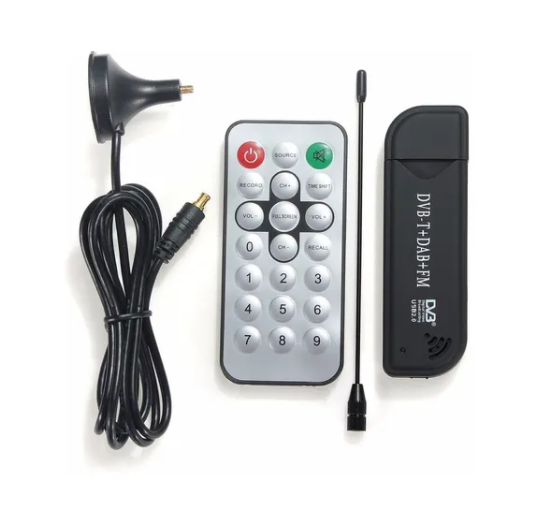
\includegraphics[scale=0.4]{sdr.png}
	\caption{Software Defined Radio utilizado para tomar las primeras mediciones}
	\label{SDR}
\end{figure}

En la figura \ref{llaves} podemos observar las primeras mediciones tomadas. Aquí podemos distinguir la estrategia de transmisión que se
utiliza. En un comienzo la señal posee un preámbulo, el cual es utilizado por el receptor para sincronizar el reloj del receptor  para 
decodificar correctamente los paquetes del transmisor. Después del preámbulo hay una palabra de sincronización que se utiliza para evitar 
choques con otros dispositivos que operan en esa banda y por último se encuentra la señal de código real.\\
Al presionar el botón del control remoto el preámbulo es enviado una única vez y luego se envía la palabra de sincronización y el
comando de acción repetidamente hasta que se deje de accionar.

\begin{figure}[htb]
	\centering
	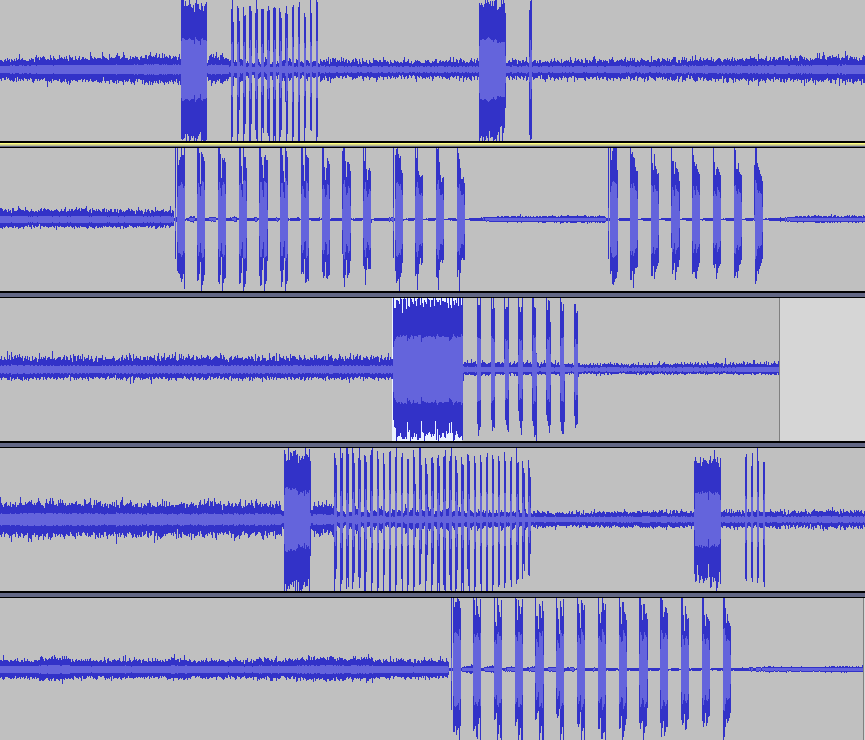
\includegraphics[scale=0.4]{llaves.png}
	\caption{Demodulación ASK de señales de controles remotos en 433,92 MHz}
	\label{llaves}
\end{figure}

\subsection{Tipos de inhibiciones}

Un inhibidor, o en inglés jammer, es un dispositivo desarrollado con el objetivo de deteriorar la comunicación en un enlace de 
radiofrecuencia. Este objetivo puede ser logrado mediante dos estrategias:

\begin{itemize}
    \item Inhibición por corrupción de datos
    \item Inhibición por saturación de etapa receptora

\end{itemize}

\subsubsection{Inhibición por corrupción de datos}

El ataque más evidente que se presenta para inhibir una comunicación es el de inyectar en el canal que se desea perjudicar una señal con 
datos aleatorios que perjudique la relación señal ruido (SNR) y dificulte la recepción para el sistema. \\
En el caso particular de los vehículos, los receptores de radiofrecuencia que se utilizan y sobre los que basamos nuestro análisis
son de 433,92 MHz con un filtro de ancho de banda de entrada de 300 KHz -como se puede observar en \todo[inline, inlinewidth=9cm, noinlinepar]{[1] AGREGAR REF A datasheet de MAX147}-.\\
El ancho de banda de recepción da lugar a sumar ruido en el canal, alterando así los datos recibidos por el demodulador. Una figura
ilustrativa se puede observa en la imagen \ref{fpb_jam} de \todo[inline, inlinewidth=9cm, noinlinepar]{referencia a carhackerhandbook [2]}.

\begin{figure}[htb]
	\centering
	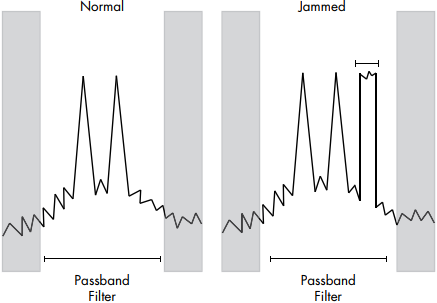
\includegraphics[scale=0.8]{fpb_jam.png}
	\caption{Presencia de inhibidor en ancho de banda de recepción}
	\label{fpb_jam}
\end{figure}

Existen diversas alternativas para efectivizar este tipo de interferencias. En la figura \ref{fpb_jam} se observa que se ha inyectado una
interferencia de ancho de banda angosto, pero también podría sumarse un tono, multitonos o sumar una señal de gran ancho de banda que 
tape completamente el canal. \\
Las alternativas antes mencionadas hacen referencia a inhibidores no inteligentes, los cuales están metiendo ruido constantemente. Hay otras 
alternativas de inhibiciones que de manera continua están escuchando el canal y cuando detectan una señal que 
desean interferir comienzan a emitir el ruido - en los papers \todo[inline, inlinewidth=3cm, noinlinepar]{[3]-[5]} se detallan
los métodos inteligentes más utilizados-. 

\subsubsection{Inhibición por saturación de etapa receptora}

Los receptores de radiofrecuencia usualmente están diseñados asumiendo que se recibirá una pequeña señal de entrada, por lo que la primer
etapa presente es un amplificador de bajo ruido.  Este es clave para que el ruido del mezclador no afecte la relación señal ruido de las 
etapas siguientes. Entre las especificaciones importantes de dichos amplificadores de RF se incluyen la figura de ruido, la ganancia y la 
intercepción de intermodulación de tercer orden.\\
La influencia de grandes señales de interferencia se manifiesta de varias formas. Una de estas es en la intermodulación de tercer orden en 
la que dos señales, una pequeña (de interés) y la interferente (de gran amplitud), se superponen. La interferente podría saturar el receptor
de modo que la señal de interés presente una pequeña ganancia. Este efecto es causado por la no linealidad de tercer orden del sistema y la relación
entrada salida está regida por \ref{eq:tercer_orden}

\begin{equation}\label{eq:tercer_orden}
    y(t) \approx  a_1 x(t) + a_2 x^{2}(t) + a_3 x^{3}(t) 
\end{equation}

Donde \emph{y} es la salida del sistema y \(a_1, a_2, a_3 \) son coeficientes. Ahora supongamos que la entrada, como es de esperar con lo antes
descripto, es \(x(t)=V_1 cos(\omega_1 t)+ V_2 cos(\omega_2 t)\), \(V_1\) representando a la señal de interés y \(V_2\) a la interferente.\\
Reemplazando en la ecuación \ref{eq:tercer_orden} y asumiendo que la interferencia es mucho más grande que la señal, la salida del sistema 
en la frecuencia de interés \(\omega_1\) resulta ser \ref{eq:intermodulacion}

\begin{equation}\label{eq:intermodulacion}
    y(t) \approx \left( a_1 x(t) + \frac{3}{2} a_3 V_2^{2} \right) V_1  cos(\omega_1 t)
\end{equation}

Para que el sistema comprima la ganancia, como es evidente que sucede, el producto \(a_1 a_3 < 0\). De aquí se puede observar entonces que
la salida del sistema en la frecuencia deseada es función de \(V_2^{2}\) y que la ganancia decae, saturando el sistema y decrementando la SNR.
Esto es fácilmente observable en la figura \ref{no_linealidad_e_tercer_orden}

\begin{figure}[htb]
	\centering
	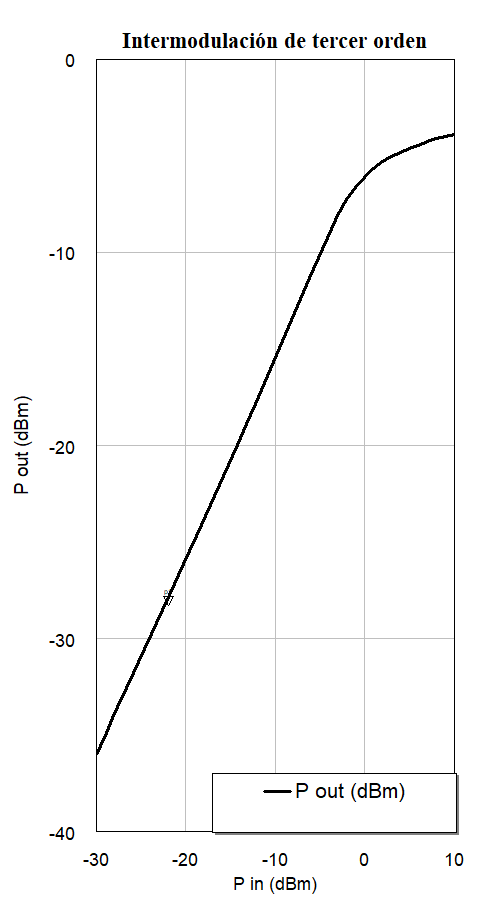
\includegraphics[scale=0.4]{no_linealidad_e_tercer_orden.png}
	\caption{Compresión de la ganancia por no linealidad de tercer orden}
	\label{no_linealidad_e_tercer_orden}
\end{figure}


\section{Objetivos de la investigación}
En base a la información recolectada establecemos los
capacidad de detectar inhibicion de potencia o corrupcion
Una forma de atacar la señal de un llavero es atascándola pasando datos basura dentro de la banda de paso del receptor RFID, 
el área en la que el receptor está escuchando una señal válida (pagina 217 imagen)




\pagebreak




\end{document}

% vamos a resoetar estas estructura: http://www.cyta.com.ar/biblioteca/bddoc/bdlibros/guia_tesis/guia_tesis_archivos/principal.htm 
% buenisima guia de latex aplicada a tesis http://minisconlatex.blogspot.com/2011/04/como-escribir-una-tesis-con-latex.html